\chapter{Analysis} \label{chp:analysis}
In order to develop an architecture that eliminates the limitations listed in section \ref{sec:existingsystem:limitations}, an analysis has been done to extract the requirements for the new software components to be used in the new architecture.
This section will constitute an analysis to such a degree that the Design chapter can discuss which protocol(s) to use and how the software components should be structured. This chapter starts by listing the assumptions made throughout the project and the proceeds with an analysis of MCLURS and the streaming idea described in section \ref{sec:streamingidea}.

% In order to develop and implement programs to send and receive streams, the requirements from the use cases must be extracted. Some requirements will be logical consequences or decisions in order to nail down details.

\todo{Uses "pub/sub pattern and "topic" " in Streaming idea}

\section{Assumptions}
During the Analysis, Design and Implementation sections the following assumptions have been made:
\begin{itemize}
	\item No packets are lost or corrupted during transmission. This assumption must hold in relative small wired networks where no WIFI is in use. From this assumption, no retransmission of packets will be implemented, and no checksum will be calculated.
	\item No bandwidth limitation exists on the network. Since most network equipment and Ethernet cables are 1 Gbit/s, and this system concerns with streams that consumes $\approx$ 48 Mbits/s(6MB/s see section \ref{sec:exisingsystem:hardware}), this 1 Gbit/ limitation is ignored. This means, that network congestion is implemented. 
	
	\item No security is taken into consideration.
		\begin{itemize}
			\item It is assumed that no data cannot tolerate getting eavesdropped.
			\item No device on the network tries to tamper with the data.
		\end{itemize}
\end{itemize}

These assumptions are discussed in chapter \ref{chp:discussion}. 

\section{Terminology} \label{sec:analysis:terminology}
Some terminology most be introduced, in order to help the reader throughout the analysis section. Figure \ref{fig:analysis:terminology} shows how data is produced by a \program{Producer}, made into a stream by a \program{Publisher} and streamed to a multicast group. The stream is then received by a \program{Subscriber} which provides the \program{Consumer} with the data originally originating from the \program{Producer.}

\begin{figure}[h!]
	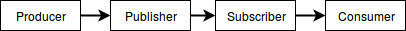
\includegraphics[width=1\textwidth]{figures/analysis-terminilogy-overview.png}
	\caption{Overview of nodes, to help the reader understand the terminology used throughout the following sections. It should be noted, that the producer and consumer is just programs producing and consuming streams without being aware of the protocols between the publisher and subscriber.} \label{fig:analysis:terminology}
\end{figure} \todo{Update figure to follow text above.}


%All nodes that publish or subscribe is stateless with respect to the data streams. However, they might both maintain a state about the metadata streams.

\todo{Assumption, no risk of getting hacked in assumptions}

\section{Streams} \label{sec:analysis:streams}
A stream is defined as "A sequence of digitally encoded signals used to represent information in transmission"\citep{data_stream_2018}. A stream does not conceptually have an explicit beginning or end nor does it necessarily have a header explaining the content of the stream.\\
From the uses cases, recordings are finite or potentially infinite streams in short and long recordings, respectively. This implies that streams should be capable of transmitting   continuous media. From \ref{sec:usecase:processing}, a stream can also consist of asynchronous events, implying streams also must be capable of transmitting discrete media. 
A stream can therefore either be continuous or discrete. 
Given use case \ref{sec:usecase:x}, a stream must be capable of comprising one of different media such as sound, text or data only by relying on available codecs. 

As mentioned in \nameref{sec:streamingidea}, the streams should be transported over multicast groups in order to distribute the streams to those network nodes that want it. 
As a logic consequence of using multicast groups, the streams must be transmitted over a  packet-oriented protocol namely UDP. Even though no packet loss is assumed, the stream must be the stream must be robust to UDP packets turning up in the wrong order, without loosing global knowledge of the stream. TCP is not an option, as this would not take advantage of the multicast groups. TCP is connection-oriented meaning it would require a connection from each \program{Publisher} to each \program{Subscriber} which would limit the number of \program{Subscribers} per \program{Publisher} due to the RPi's bandwidth limitation.
 
%As all streams are transmitted over multicast groups, the streams must be packet-oriented since they are transported as UDP packets.

As the stream is just data, there must be metadata available that describes the content of the streams. The streams must be described unambiguously, such that each stream can be differentiated from other streams. The streams must therefore be self-identifying meaning when a subscriber receives a stream, it should already know the properties of the stream such as the media of the stream. The streams must not rely on codecs or formats that put metadata in the beginning of the stream, as this would assume \program{Subscribers} always receive the beginning of a stream, which should not be the case.

Since the streams are to be recorded and replayed, metadata must also be available when the streams are replayed, in order to identify the streams when replayed. Therefore, the streams must be complete and depend on no external knowledge. Analysis of the metadata is conducted in section \ref{sec:analysis:metadata}. When a stream is replayed, it should not necessarily be recorded again. This implies the streams associated metadata must state if the stream should not be recorded.

As the system will usually comprise of multiple streams, each stream must have a unique, sensible name used to refer to the stream. Furthermore it must have an unique identifier that allow streams to refer to each other.
As in use case \ref{sec:usecase:energizer}, where a node consumes a stream and produces a new stream, the new stream must explicitly specify its parent stream using the parent's unique identifier. This gives rise to model the streams as a forest of graphs, where each graph should always be an directed acyclic graph, in order to avoid streams that depend on themselves. An example graph is shown in figure \ref{fig:analysis:graph}

\begin{figure}[h!]
	\centering
	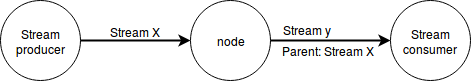
\includegraphics[width=1\textwidth]{figures/stream-graph}
	\caption{Graph of streams} \label{fig:analysis:graph}
\end{figure}\todo{Update name in nodes}

Requirements extracted from the analysis are listed in table \ref{tab:requirements}.

\section{Metadata} \label{sec:analysis:metadata}
\subsection{Introduction}

By inspection of the use cases and the streaming analysis in section \ref{sec:analysis:streams}, it has been decided to split metadata into tree categories:
\begin{enumerate}
	\item \textit{Essential metadata} which covers the metadata that is required to identify and decode the stream.
	\item \textit{Non-essential metadata} which is used between the producer and consumer. This metadata is only relevant to the users.
	\item \textit{Events} which describes an event in the stream. An event is defined as something interesting in the stream.
\end{enumerate}

When "metadata" is used, it refers to Essential and none-essential metadata.
\subsection{Event} \label{sec:analysis:event}
From section \ref{sec:dataanalysis}, it is required that events consists of a timestamp, duration and data. The system must therefore handle events consisting of the following entries:
\begin{itemize}
	\item \textit{Start} States the absolute date and time of when the event appear. 
	\item \textit{Duration} States for how long time the event is active.
	\item \textit{Data} Associates data to the event. 
\end{itemize}

Given that streams are to be recorded replayable, the events must also be replayable while still relating to a stream and point in time explicitly and unambiguously.

\subsection{Essential Metadata} \label{sec:analysis:essentialmetadata}
From the analysis of streams~\ref{sec:analysis:streams}, it is required that the streams are self-identifying to the \program{Subscriber}. This implies that metadata that describes the properties of the stream must be available to the subscriber.
From the analysis of streams ~\ref{analysis:stream:requirement:x}, it is required that subscribers can join a stream at any arbitrary time.\todo{Followup on this} In order for the \program{Subscriber} to know the properties of the stream, the metadata must be retransmitted periodically. This metadata is essential in order to identify and decode the stream and will be referred to as "essential metadata". When a stream is replayed, the associated metadata must explicitly state if the stream should not be recorded.

\subsubsection{Metadata Format}
The metadata format must be extensible such that the structure and list of parameters can be modified later on as needed.

It has been decided that metadata is essentially hierarchical key-value structures, that can be represented in different formats such as XML, JSON, EBML etc.  From that decision it follows, that metadata is:
\begin{itemize}
	\item Extensible - as new key-value pairs can be added as needed.
	\item Expressive - since associative arrays, arrays etc. can be expressed.
	\item Convertable - as both \program{subscribers} and \program{Publishers} can convert into the format required by the \program{Consumer} and \program{Publishers} independently.
\end{itemize}

\subsection{None-essential Metadata}
\ac{MCLURS} provides metadata about the streams, which is not essential to identify or decode the stream but is relevant to the user. An example of none-essential metadata is listed in section \ref{sc:existingsystem:setup}.
The publishers and subscribers must be agnostic to the format and semantics of this metadata, as it is provided by the \program{Producer} and used by the \program{Consumer}. The subscriber and publisher must allow for conversion between different formats used by the producer and consumer, in order to ease implementing \program{Producers} and \program{Consumers}.
%The subscriber and publisher must also be agnostic to the format of the metadata, as the producer and consumer might use XML, JSON, EMBL etc. to represent metadata.
This will be referred to as "none-essential metadata", as this metadata is not essential with respect to the streams.\\

\section{Publishers \& Subscribers} \label{sec:analysis:pubsub}
\subsection{Introduction}
The terminology used to describe types of streams throughout this analysis is used from RFC7656\citep{RFC:7656}.

%Nodes publishing streams will be referred to as publishers through the following sections. Nodes receiving streams will be referred to as a subscriber, as they subscribe to streams in order to get the streams. \\
A \program{Subscriber} and \program{Publisher} is depicted in figure~\ref{fig:analysis:pubsub}.

\begin{figure}[h!]
    \centering
    \begin{subfigure}[b]{1\textwidth}
        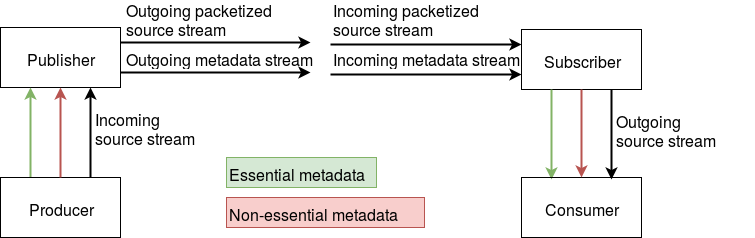
\includegraphics[width=\textwidth]{figures/publisher-subscriber}
    \end{subfigure}
     \caption{A publisher(left) and subscriber(right) depicted}\label{fig:analysis:pubsub}
\end{figure}

A source stream is defined as a stream of digital samples that has been synchronized with a reference clock and comes from a particular media source.

A packetized source stream is defined as a source stream where the stream is split into packets.
The outgoing source stream is identical to the incoming source stream.
Non-essential metadata is as defined in \ref{sec:analysis:metadata}. Incoming none-essential metadata will be the same key-value pairs as the outgoing none-essential metadata.

The \textit{outgoing metadata stream} is \textit{none-essential} and \textit{essential metadata} combined as \textit{essential metdata} is used by the \program{Publisher} and \program{Subscriber}.

\subsection{Analysis} \label{sec:analysis:pubsup:introduction}
As streams may contain different media, the \program{Publisher} and \program{Subscriber} must be agnostic to the codec of the stream, and must provide an interface to handle the data as well as metadata to and from the streams.
In order to allow multiple nodes to use a stream, multiple \program{Subscribers} must be able to subscribe to the same multicast group. If a \program{Publisher} publishes to a topic already in use, it must give a warning to the user. In order for this to work, the publishers and subscribers must implement a presence protocol, that detects the presents of other \program{Publishers} and \program{Subscribers} on a specific stream. This must be implemented in a way such that possible conflicts can be detected within X seconds from a publisher/subscriber is run, where X is specified as a parameter to the nodes.

As there is no designated master in the system, the publisher must be designed such that that independently can find available multicast groups, without relying on too many well-known multicast groups. When a subscriber is told to subscribe to a stream using the stream's unique name, the subscriber must single-handedly be able to find the requested multicast group.
As publishers and subscribers unlikely joins multicast groups at the same time, the publisher and subscriber most be able to cope with nodes asynchronously joining and leaving multicast groups.

Given design requirement X in section \ref{sec:analysis:designrequirements}, the publishers/subscribers must be opaque such that they encapsulate all of their internal protocols. In practice this means that the producers and consumers must be unaware of the communication between the \program{Subscribers} and \program{Publishers}.

%Both producer and consumer must be implemented as C-libraries and support bindings to other languages, to ease implementing new consumers and producers for future applications.

%The publishers and subscribers must react to

As metadata is required, it must be possible to provide metadata to the \program{Publishers} such that it can stream it to the \program{Subscribers}.
Given that the \program{Subscribers} and \program{Publishers} work on incoming data from either a stream or \program{Producer}, they should only do work if 1) data from a stream is received or 2) the node must do work periodically such as send metadata.

\section{Historian} \label{sec:analysis:historian}

Storing data is essential in all use cases, that require post-processing of recordings. Saving recordings to a local disk and later replaying the recordings should be the only responsibilities of a designated node referred to as \program{Historian}.
The \program{Historian} should not be limited to record one stream, but should be capable of saving recordings from multiple streams. 

The historian should be able to save the  three types of recordings, as described in section~\ref{sec:usecase:recordingtypes}:
\begin{itemize}
	\item Long recordings
		In order for the node to save long recordings, it should be capable of writing to a local mounted storage periodically, and not store the entire recording in memory, as this would limit the maximum recording time.

	\item Short recordings
		With short recordings, the same applies as longtime recordings, however it should be possible to decide when and for how long time the recording should run. The historian must provide an interface that allows setting when to do recordings and for how long time.
	\item Trigger recordings
		From use case \ref{usecase:trig}, trigger recording is required. The \program{Historian} must be able to replay a recording of arbitrary length at a arbitrary time of recorded data. This implies that the \program{Historian} must support recording while replaying recordings. For this to work, it must be possible to specify which interface the \program{Historian} should replay the recordings to.
\end{itemize}

As the node should be responsible for recording multiple streams, it should save the streams unambiguously with their associated metadata, such that the streams can be uniquely identified when replayed.
Given that streams can contain different media, the \program{Historian} must be agnostic to the content of the stream and to the None-essential metadata.

Given that it might be possible that a stream must not be recorded, the \program{Historian} must support ignoring streams that explicit states not to be recorded.

\subsection{Replaying}
As introduced in section \ref{sec:streamingidea}, nodes processing streams can either be run when the recordings are happening(online) or when the streams are replayed(offline). In order for this to work, the \program{Historian} must replay streams such that the processing nodes are unaware of the streams are online or offline. This further implies that the content of the streams must be replayed in same order as it was recorded and support real-time replaying meaning x seconds of recording takes x seconds to replay. Furthermore, this implies that metadata recorded must be replayed with the streams. From section~\ref{sec:streamingidea} it is required to be able to replay the same recordings multiple times. This implies that the historian must not delete the recordings after the recording has been replayed the first time.
As the \program{Historian} saves streams and metadata with respect to time, the replaying must be started by requesting a replay from a given time and date. It should also be possible to request for how long a period the \program{Historian} should replay streams, so that a replay will not continue forever. For this to work, the historian must have an interface that allows requesting the following options:

\begin{itemize}
	\item Date and time from where the historian should replay the streams.
	\item Selecting which streams to be replayed.
	\item To which interface the streams should be replayed. This will be useful in the use case \ref{usecase:trigger}, where requesting data might happen meanwhile the historian is recording.
	\item Replay rate that allows setting how fast the replaying should happen. 
\end{itemize}

As there is no guarantee that all \ac{MCLURS} RPis are powered up when the historian starts recording, the historian must be able to autodiscover streams as they become available using the presence mechanism described in section \ref{sec:analysis:pubsub}.

The historian should not rely on specific hardware configuration. See section \ref{section:analysis:network} for analysis of required network.


From the analysis, the following requirements are extracted.
\begin{enumerate}
	\item The historian must support recording multiple streams to local mounted storage.
	\item The historian must support replaying while recording.
	\item The historian must be agnostic with respect to the streams' encoding.
	\item The replayed streams must be unambiguous.
	\item The historian must replay streams with all of the streams' associated metadata.
	\item The historian must be robust to stream packets arriving out-of-order or never arriving.
	\item The historian must replay streams' packets in same order as they are recorded.
	\item The historian must ignore streams that explicitly states they should not be recorded.
	\item The historian must be able to replay streams and metadata in real-time, as they are recorded.
	\item The historian must not change the stream nor metadata during replaying.
	\item The historian must replay streams such that a processing-node cannot tell whether the stream is replayed or live.
	\item The historian must support replaying the same stream multiple times.
	\item The historian must have an interface that allows requesting:
	\begin{itemize}
		\item Date and time from where the historian should replay the streams.
		\item Selecting which streams to be replayed.
		\item To which interface the streams should be replayed. 
		\item Replay rate that allows setting how fast the replaying should happen. 
		\item How many packet should be replayed.
		\item When the historian should record and for how long time.
	\end{itemize}
	The historian must not rely on specific hardware with specific properties.
	The historian must be able to discover streams as the streams appear on the network.
\end{enumerate}

Given the limited time, the requirements has been prioritized into \textit{Need to have} and \textit{Nice to have} in table \ref{sec:analysis:historian:tablefeatures}.
\begin{table}[h!]
\centering
\caption{Table prioritizing the requriements into nice-to-have and must-have}
\label{sec:analysis:historian:tablefeatures}
\begin{tabular}{l|l|l}

\multicolumn{3}{l}{Need to have}              \\ \hline
----------  & --------- & ---------------------------------- \\ \hline
----------- & --------  & --------------------------------- \\ \hline
\multicolumn{3}{l}{Nice to have}              \\ \hline
            &           &                       \\ \hline
            &           &                       \\ \hline
\end{tabular}
\end{table}

\section{Energy Calculator} \label{sec:analysis:energy}
\textbf{Just some notes}
% Node responsible for calculating energy in signal. 
From use case \ref{sec:usecase:energizer}, the energy calculation should happen from bulk of samples corresponding to 1 ms. To ease the implementation of the energizer-node and future nodes, it should be possible to set the payload size of the publisher node. If the payload length of the stream corresponds to 1 ms of samples, the energizer node do not have to implement a buffer mechanism. If the length of the packet exceeds the practical limits of the network, the producer must give a warning. From the incoming data to the producer, and the outgoing data from the consumer, there should be no limit of the packet sizes.

\section{Network} \label{sec:analysis:network}
%As all streams leaving the nodes are timestamped, there are no restrictions on how the devices should be connected on the network. Packets can go through different number of hobs without causing problems, if the timestamps from the streams are used, and not the order the packets are leaving the historian during replay.

%To connect multiple hosts on the network, multiple switches can be connected together. If multiple switches are connected, the bandwidth between switches should be handled with care. Each batbox generates 40 Mbit/s of data, so if a 24 ports switch is used to connect 23 batboxes and one historian, the link between the switch and the \program{Historian} must be 1 Gbit. If an 48 ports switch is used, 1.8 Gbits is required between the switch and the \program{Historian}. A switch's non-blocking capacity, meaning the bandwidth it can handle at the same time, not always equals the (number of ports) x (the bandwidth of each port).
As stated in \ref{sec:streamingidea}, multicast is used to distribute streams to \program{Subscribers}. The streams could instead be broadcasted, which would cause all devices on the network to receive the streams. This is usually unwanted, as this puts more load on the network that needed. All network attached devices would have to drop the streams, unless they want it. Unicast is also an option, but this would imply that a publisher would have to send N streams if N subscribers subscribes to a stream which would put unnecessary load on the publisher and the network.

As multicast is utilized to distribute streams, each switch must support the following features in order to handle multicast traffic properly.

\begin{itemize}
	 \item IGMP snooping, in order to avoid broadcasting multicast traffic.
	 \item MLD, protocol used by IPv6 to join and leave multicast groups.
\end{itemize}
If IPv6 is used, the switches most support both features, otherwise only IGMP snooping is required. If IGMP snooping is not supported, the multicast traffic will be broadcasted to all network attached devices.

If the system scales out enough, limitations might arise, however these are not seen as realistic limitations.

\subsection{Loopback Multicast Traffic} \label{sec:analysis:localmulticasttrafic}
As in use case \refname{sec:usecase:drone} where a single RPI is used, the \program{Historian} must run on the same RPi is the \ac{MCLURS} software. In order for this to work, the multicast traffic most also work on a loopback interface. 

\subsection{Requirements}
From the analysis, the following requirements are extracted.
\subsubsection{Streams}
\begin{enumerate}
	\item The stream can be either continuous or discrete.
	\item The stream must comprise different datatypes only by relying on available codecs.
	\item The stream must be packet-oriented and stateless
	\item The stream must be transported over UDP
	\item The stream must be robust to UDP packets that arrive out of order or never arrive.
	\item The stream must be represented unambiguously
	\item Metadata must be provided by the publishers and be available to the subscribers 
\end{enumerate}
\todo{Table of requirements[Where it's defined][Where it's tested][Whether it passes}

\subsubsection{Publisher \& Subscriber}
\begin{enumerate}
	\item The \program{Publisher} and \program{subscriber} must be agnostic to the stream's payload.
	%\item Multiple producers must send to the same multicast group.
	\item Multiple \program{Subscribers} must receive from the same multicast group.
	\item The \program{Publishers} and \program{Subscribers} must implement a presence mechanism to know about other \program{Publishers} and \program{Consumers}.
	\begin{enumerate}
		\item It must takes a finite maximum number of seconds for a \program{Publisher} or \program{subscriber} to know who is present in a stream. The max time must be a parameter of each node.
		\item It must take a finite maximum number of seconds for a \program{Publisher} or \program{Subscriber} to detect whether a multicast group is in use, and if yes, by whom.
		\item It must assume nodes leaving a multicast group sends a "bye".
		\item It must be robust to "bye"-messages not arriving to all nodes.
		\item It must handle nodes joining and leaving at any arbitrary time.
	\end{enumerate}
	\item The \program{Publishers} must be able to find unused multicast groups single-handedly.
	\item Given a unique name of a stream, the \program{Subscriber} must be able to resolve the multicast address of the stream.
	\item Both \program{Publishers} and \program{Subscribers} must be able to cope with nodes joining asynchronously.
	%\item The producer and consumer must be implemented in C and support language bindings.
	\item The payload length of the stream should be adjustable as a parameter on the \program{Publishers}.
		\begin{enumerate}
			\item If the requested payload size is exceeding practical limits, a warning must be given.
		\end{enumerate}
	%\item There should not be a limit of the packet size of the incoming data to the producer, or outgoing data from the consumer.
	\item Metadata provided by a \program{Producer} must be streamed to \program{Subscribers}.
	\item Both \program{Subscribers} and \program{Publishers} must be agnostic with respect to the semantics and format of the none-essential metadata.
\end{enumerate}

\subsubsection{Metdata}

\begin{enumerate}
	\item Metadata must unambiguously relate to the streams.
	\item Metadata must be expressive.
	\item Metadata must be convertable.
	\item Metadata must be extensible.
	\item Metadata must be complete.
	\item Metadata must be hierarchical key-value pairs.
	\item The \program{Publishers} and \program{Subscribers} must be capable of converting between metadata formats.
	\item Events must have a start time and date
	\item Events must have a duration.
	\item Events must contain data relating to the event.
	\item Essential metadata must be retransmitted periodically
	\item None-essential metadata must be retransmitted periodically
\end{enumerate}

\subsubsection{Historian}
